\documentclass[tikz, border=5mm]{standalone}
\usepackage[utf8]{inputenc}
\usepackage[T1]{fontenc}
\usepackage{lmodern}
\usetikzlibrary{shapes.geometric, positioning, calc, backgrounds, arrows.meta}

\begin{document}
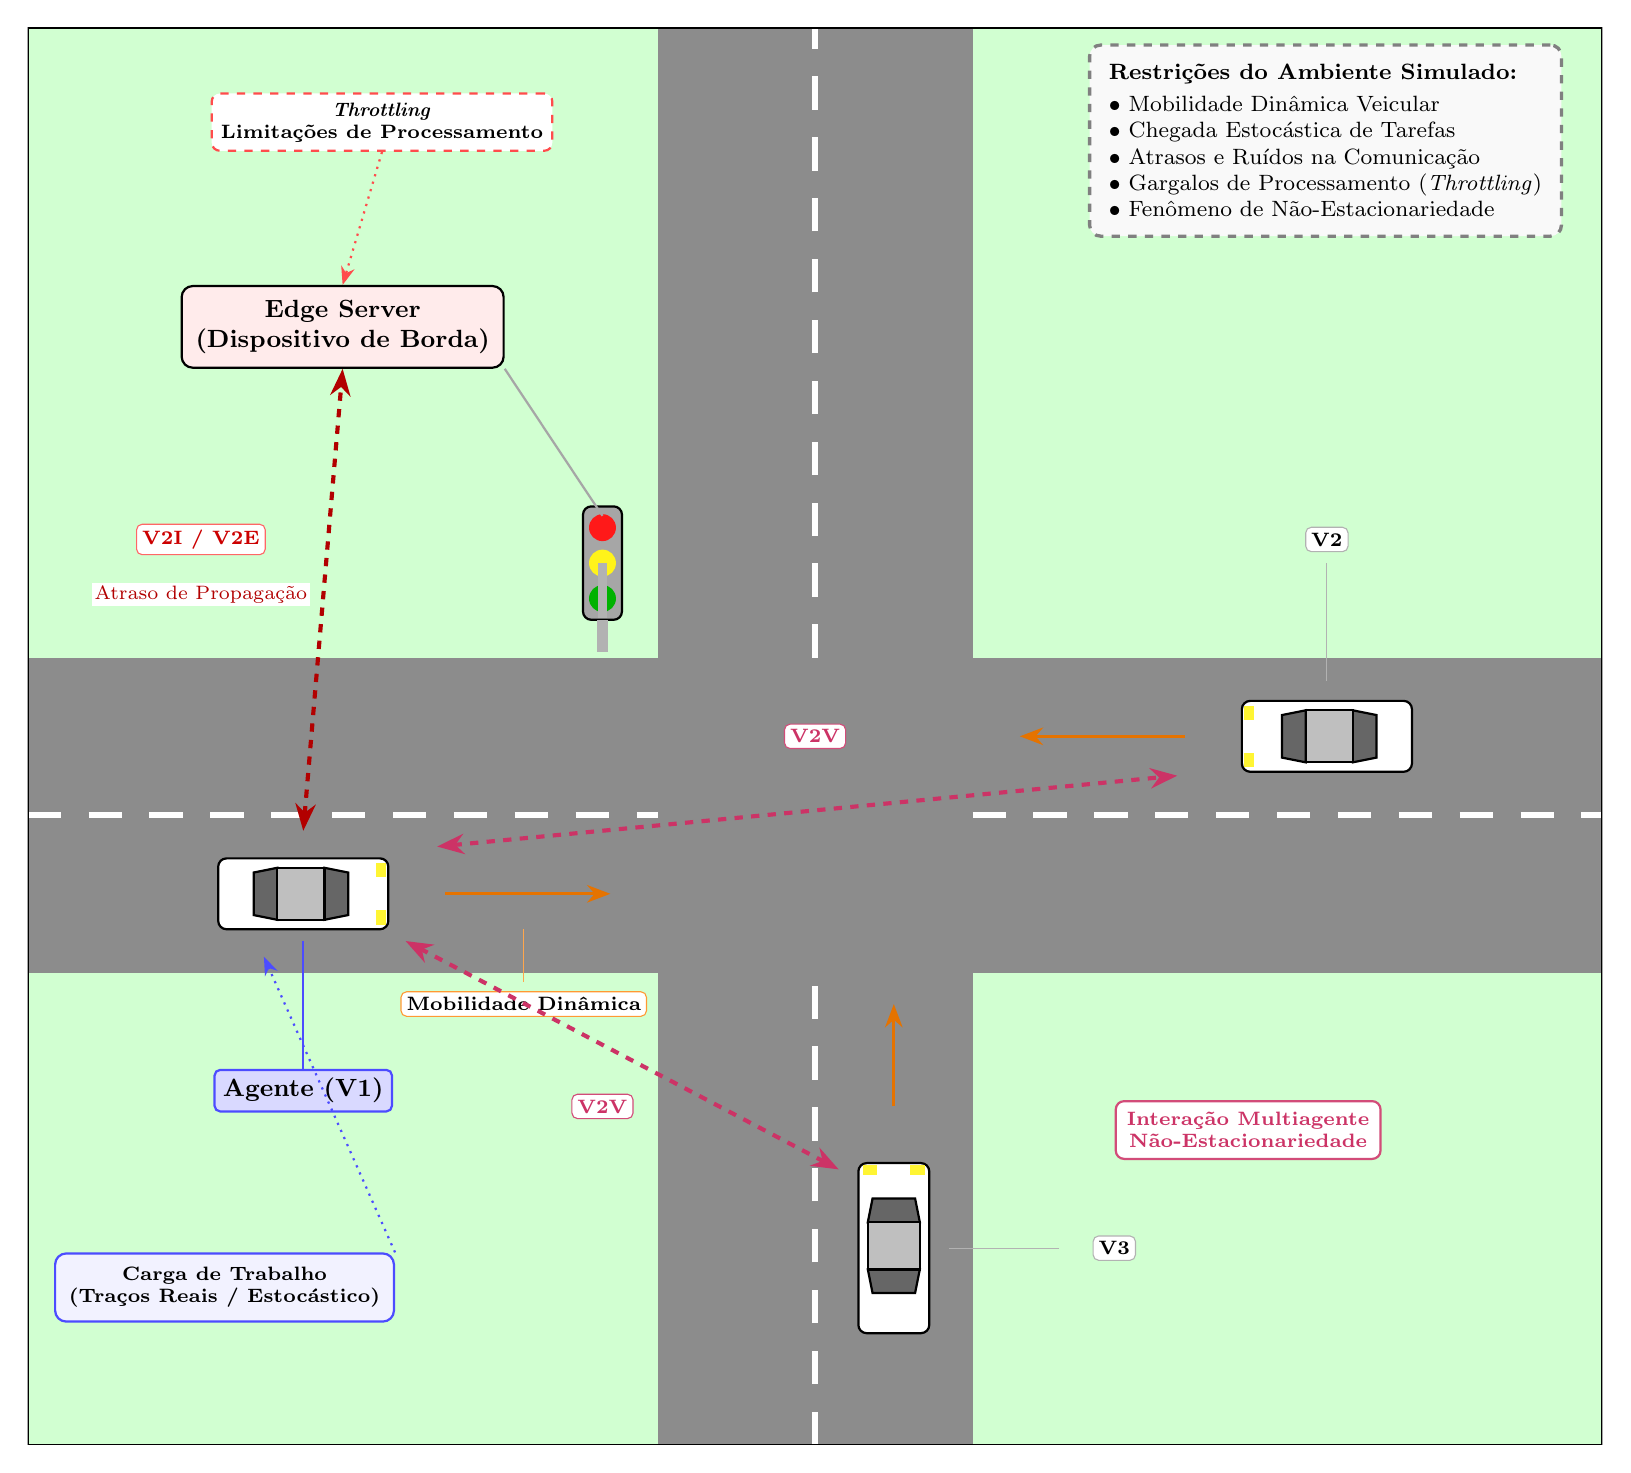
\begin{tikzpicture}[
    font=\sffamily,
    >=Stealth,
    car right/.pic={
        \begin{scope}[scale=0.6]
            \filldraw[fill=white, draw=black, rounded corners=3pt, thick]
                (-1.8,-0.75) rectangle (1.8,0.75);
            \filldraw[fill=black!60, draw=black, thick]
                (-0.55,-0.55) -- (-1.05,-0.45) -- (-1.05,0.45) -- (-0.55,0.55) -- cycle;
            \filldraw[fill=black!60, draw=black, thick]
                (0.45,-0.55) -- (0.95,-0.45) -- (0.95,0.45) -- (0.45,0.55) -- cycle;
            \filldraw[fill=black!25, draw=black, thick]
                (-0.55,-0.55) rectangle (0.45,0.55);
            \filldraw[fill=yellow!80, draw=none]
                (1.55,-0.65) rectangle (1.75,-0.35);
            \filldraw[fill=yellow!80, draw=none]
                (1.55,0.35) rectangle (1.75,0.65);
        \end{scope}
    },
    car up/.pic={
        \begin{scope}[scale=0.6]
            \filldraw[fill=white, draw=black, rounded corners=3pt, thick]
                (-0.75,-1.8) rectangle (0.75,1.8);
            \filldraw[fill=black!60, draw=black, thick]
                (-0.55,-0.45) -- (-0.45,-0.95) -- (0.45,-0.95) -- (0.55,-0.45) -- cycle;
            \filldraw[fill=black!60, draw=black, thick]
                (-0.55,0.55) -- (-0.45,1.05) -- (0.45,1.05) -- (0.55,0.55) -- cycle;
            \filldraw[fill=black!25, draw=black, thick]
                (-0.55,-0.45) rectangle (0.55,0.55);
            \filldraw[fill=yellow!80, draw=none]
                (-0.65,1.55) rectangle (-0.35,1.75);
            \filldraw[fill=yellow!80, draw=none]
                (0.35,1.55) rectangle (0.65,1.75);
        \end{scope}
    },
    semaforo/.pic={
        \begin{scope}[scale=0.45]
            \filldraw[fill=gray!70, draw=black, thick, rounded corners=3pt]
                (-0.55,-1.6) rectangle (0.55,1.6);
            \fill[red!90] (0, 1.0) circle (0.38);
            \fill[yellow!90] (0, 0) circle (0.38);
            \fill[green!70!black] (0,-1.0) circle (0.38);
            \draw[gray!60, line width=4pt] (0,-1.6) -- (0,-2.5);
        \end{scope}
    }
]
    % Canvas: 20x18
    \clip (0,0) rectangle (20,18);

    % Fundo
    \fill[green!18] (0,0) rectangle (20,18);

    % Ruas
    \fill[black!45] (0,6) rectangle (20,10);
    \fill[black!45] (8,0) rectangle (12,18);
    \fill[black!45] (8,6) rectangle (12,10);

    % Marcações de faixa
    \draw[line width=2.2pt, white, dashed, dash pattern=on 12pt off 10pt] (10,0)  -- (10,6);
    \draw[line width=2.2pt, white, dashed, dash pattern=on 12pt off 10pt] (10,10) -- (10,18);
    \draw[line width=2.2pt, white, dashed, dash pattern=on 12pt off 10pt] (0,8)   -- (8,8);
    \draw[line width=2.2pt, white, dashed, dash pattern=on 12pt off 10pt] (12,8)  -- (20,8);

    % V1: Agente
    \pic at (3.5,7) {car right};
    \node[fill=blue!15, draw=blue!70, rounded corners=2pt, thick,
          font=\small\bfseries, align=center, inner sep=3pt]
        (lagente) at (3.5,4.5) {Agente (V1)};
    \draw[blue!70, thick] (lagente.north) -- (3.5,6.4);
    \draw[->, very thick, orange!90!black] (5.3,7.0) -- (7.4,7.0);
    \node[fill=white, draw=orange!80, rounded corners=2pt,
          font=\scriptsize\bfseries, inner sep=2pt]
        at (6.3,5.6) {Mobilidade Din\^amica};
    \draw[orange!70, thin] (6.3,5.88) -- (6.3,6.55);

    % V2
    \pic[rotate=180] at (16.5,9) {car right};
    \draw[->, very thick, orange!90!black] (14.7,9.0) -- (12.6,9.0);
    \node[fill=white, draw=gray!60, rounded corners=2pt,
          font=\scriptsize\bfseries, inner sep=2pt]
        at (16.5,11.5) {V2};
    \draw[gray!60, thin] (16.5,11.2) -- (16.5,9.7);

    % V3
    \pic at (11,2.5) {car up};
    \draw[->, very thick, orange!90!black] (11,4.3) -- (11,5.6);
    \node[fill=white, draw=gray!60, rounded corners=2pt,
          font=\scriptsize\bfseries, inner sep=2pt]
        at (13.8,2.5) {V3};
    \draw[gray!60, thin] (13.1,2.5) -- (11.7,2.5);

    % Semafor + Edge
    \pic at (7.3,11.2) {semaforo};
    \draw[gray!60, line width=3pt] (7.3,11.2) -- (7.3,10.5);
    \node[draw=black, fill=red!8, thick, rounded corners=4pt,
          align=center, font=\small\bfseries, inner sep=5pt]
        (edge) at (4.0,14.2) {Edge Server\\(Dispositivo de Borda)};
    \draw[thick, gray!70] (7.3,11.8) -- (edge.south east);

    % Carga de Trabalho
    \node[draw=blue!70, fill=blue!5, thick, rounded corners=4pt,
          align=center, font=\scriptsize\bfseries, inner sep=5pt]
        (workload) at (2.5,2.0) {Carga de Trabalho\\(Tra\c{c}os Reais / Estoc\'astico)};
    \draw[->, dotted, thick, blue!70] (workload.north east) -- (3.0,6.2);

    % V2I
    \draw[<->, dashed, line width=1.5pt, red!70!black]
        (3.5,7.8) -- (edge.south);
    \node[fill=white, draw=red!60, rounded corners=2pt,
          font=\scriptsize\bfseries, text=red!80!black, inner sep=2pt]
        at (2.2,11.5) {V2I / V2E};
    \node[fill=white, font=\scriptsize, text=red!70!black, inner sep=1pt]
        at (2.2,10.8) {Atraso de Propaga\c{c}\~ao};

    % Throttling
    \node[draw=red!70, fill=white, dashed, thick, rounded corners=3pt,
          align=center, font=\scriptsize\bfseries]
        (throttle) at (4.5,16.8) {\textit{Throttling}\\Limita\c{c}\~oes de Processamento};
    \draw[->, dotted, thick, red!70] (throttle.south) -- (edge.north);

    % V2V: Agente <-> V3
    \draw[<->, dashed, line width=1.5pt, purple!80]
        (4.8,6.4) -- (10.3,3.5);
    \node[fill=white, draw=purple!70, rounded corners=2pt,
          font=\scriptsize\bfseries, text=purple!80, inner sep=2pt]
        at (7.3,4.3) {V2V};

    % V2V: Agente <-> V2
    \draw[<->, dashed, line width=1.5pt, purple!80]
        (5.2,7.6) -- (14.6,8.5);
    \node[fill=white, draw=purple!70, rounded corners=2pt,
          font=\scriptsize\bfseries, text=purple!80, inner sep=2pt]
        at (10.0,9.0) {V2V};

    % Nao-Estacionariedade
    \node[fill=white, draw=purple!70, thick, rounded corners=3pt,
          align=center, font=\scriptsize\bfseries, text=purple!80, inner sep=4pt]
        at (15.5,4.0) {Intera\c{c}\~ao Multiagente\\N\~ao-Estacionariedade};

    % Legenda
    \node[draw=black!50, fill=gray!5, very thick, dashed, rounded corners=4pt,
          align=left, font=\footnotesize, inner sep=7pt, anchor=north east]
        at (19.5,17.8) {
        \textbf{Restri\c{c}\~oes do Ambiente Simulado:}\\[2pt]
        $\bullet$ Mobilidade Din\^amica Veicular\\
        $\bullet$ Chegada Estoc\'astica de Tarefas\\
        $\bullet$ Atrasos e Ru\'idos na Comunica\c{c}\~ao\\
        $\bullet$ Gargalos de Processamento (\textit{Throttling})\\
        $\bullet$ Fen\^omeno de N\~ao-Estacionariedade
    };

    \draw[thick] (0,0) rectangle (20,18);
\end{tikzpicture}
\end{document}
